\section{Funktionen}
\begin{def*}[note = Funktion , index = Funktion]
	Eine Relation $f \subseteq A \times B$ heisst \textbf{funktional} (Funktion $f: A \rightarrow B$) falls:
	\begin{gather*}
		\forall a \exists b : (a,b) \in f \\
		(a,b) \in f \wedge (a,b') \in f \implies b = b' \\
		\intertext{oder einfach:}
		\forall a \exists ! b (a,b) \in f
	\end{gather*}
	Wir schreiben für $(a,b) \in f$: \\
	$f( a ) = b , f: a \mapsto b$
\end{def*}
\begin{def*}[note = Komposition , index = Komposition]
	(Als Relationskomposition $''f \ring g''$) \\
	\begin{gather*}
		f: A \rightarrow B, g: B \rightarrow C \\
		g \ring f( a ) = g( f( a ))
	\end{gather*}
\end{def*}
\begin{def*}[note = Injektivität , index = Injektivität]
	$f: A \rightarrow B$ \textbf{injektiv}, falls \\
	$a \neq a \implies f( a ) \neq f( a' )$
\end{def*}
\begin{def*}[note = Surjektivität , index = Surjektivität]
	$f: A \rightarrow B$ \textbf{surjektiv}, falls \\
	$\forall b \exists a : f( a ) = b$
\end{def*}
\begin{def*}[note = Bijektivität , index = Bijektivität]
	$f: A \rightarrow B$ \textbf{bijektiv}, falls $f$ injektiv und surjektiv.
\end{def*}
\todo{Hyperref it up.}

\subsubsection{Die Kardinalitäten von Mengen}
\begin{def*}[note = Gleichmächtig , index = Gleichmächtig]
	\begin{gather*}
		A \preceq B, \text{ falls } \exists f : A \rightarrow B \text{ injektiv } \iff \exists g : B \rightarrow A \text{ surjektiv}. \\
		A \approx B \text{ gleichmächtig, falls } \exists f : A \rightarrow B \text{ bijektiv}.
	\end{gather*}
	Dann gilt:
	\begin{itemize}
		\item $A \approx A \quad (f = id_A)$
		\item $A \preceq B \wedge b \preceq C \implies A \preceq C$
		\item $A \preceq B \wedge B \preceq A \implies A \approx B$
		\item Totalität: $A \preceq B \vee B \preceq A$
	\end{itemize}
\end{def*}
\begin{bsp*}
	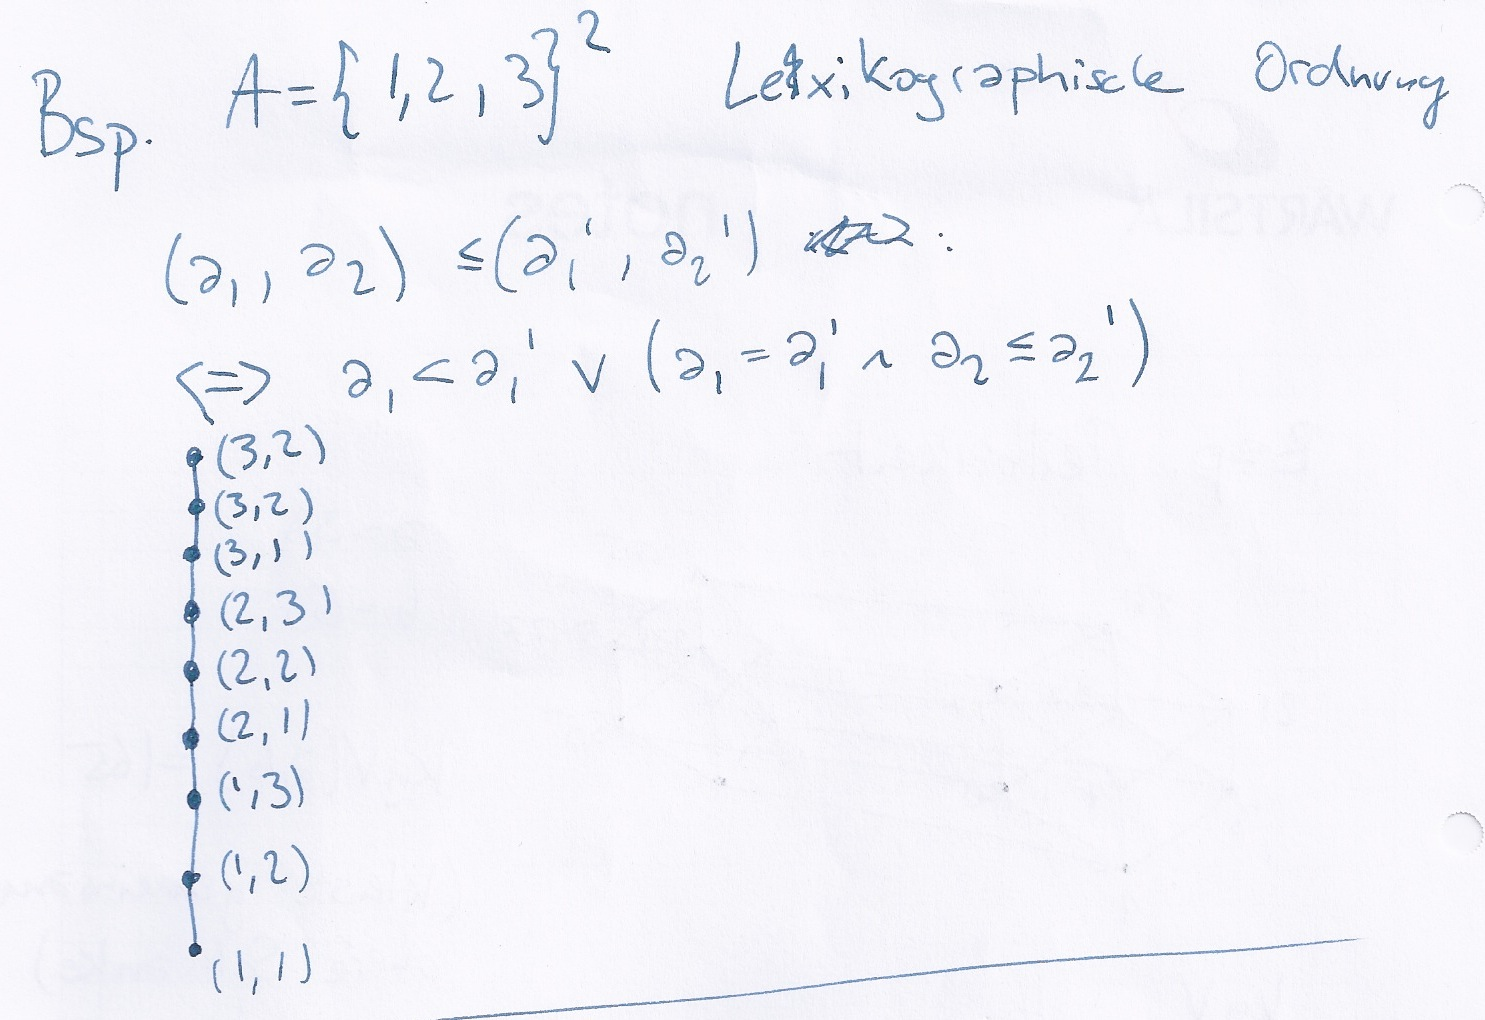
\includegraphics[width=\textwidth]{Bild23}
\end{bsp*}
\begin{satz*}[note = {(Schnöder, Bernstein, Cantor)}]
	$A \preceq B \wedge B \preceq A \iff A \approx B$\\
	\begin{bew}[note = ''Beweis'':]
		B hat eine zu A gleichmächtige Teilmenge und umgekehrt.\\
		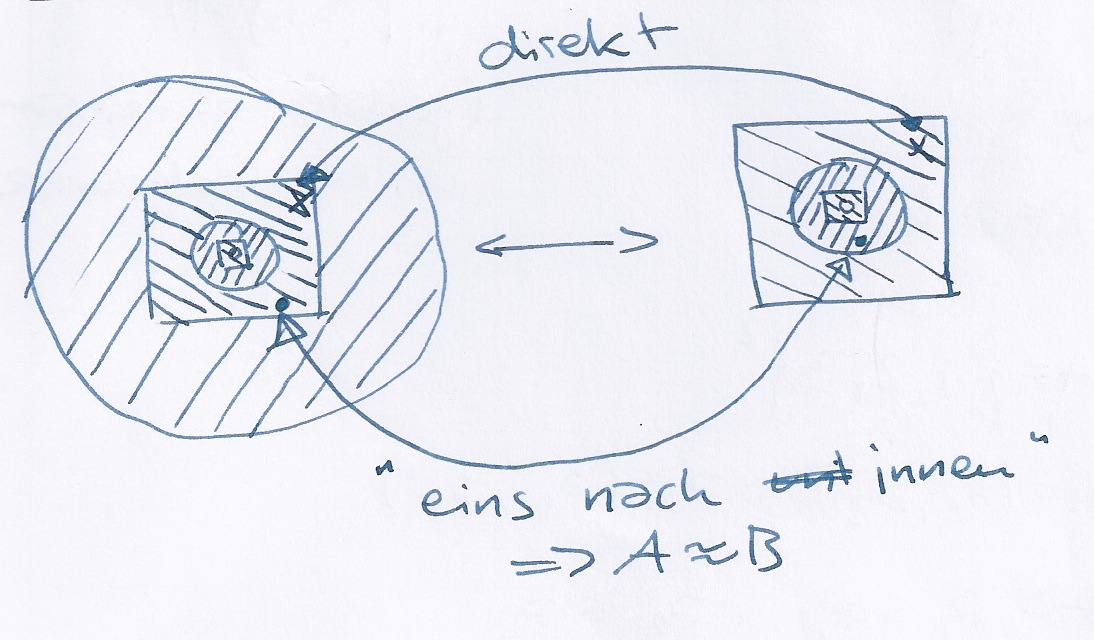
\includegraphics[width=\textwidth]{Bild24}
	\end{bew}
\end{satz*}
\begin{def*}[note = Gleichmächtigkeit , index = Gleichmächtigkeit]
	$\approx$ ist eine Äquivalenzrelation auf Klasse aller Mengen.\\
	Äquivalenklassen = Kardinalzahlen:\\
	$0, 1, 2, \dotsc , n, n+1, \dotsc \mathbb{N}, \dotsc , \mathbb{R}, \mathbb{P}(\mathbb{R}), \mathbb{P}(\mathbb{P}(\mathbb{R})), \dotsc$
\end{def*}
\begin{satz*}[note = (Cantor)]
	Für alle Mengen $A$ gilt\\
	\[ \mathbb{P}(A) \not\approx A \]
	\begin{bew}
		\begin{gather*}
			f: A \rightarrow \mathbb{P}(\mathbb{A}) \\
			\intertext{Wir zeigen: $f$ nicht surjektiv.}
			\forall a \in A : a \in f(a) \vee a \notin f(a) \\
			B \coloneqq \{ a \in A \mid a \notin f(a) \} \subseteq A, b \in \mathbb{P}(\mathbb{B}) \\
			\text{Annahme: } B = f(b) \\
				b \in B = f(b) ? \\
				b \in f(b) \implies b\notin f(b) \implies b \in f(b) \\
				\text{\lightning ~ Also } ( \not\exists f(b) = B ) \implies f \text{ nicht surjektiv } \blacksquare
		\end{gather*}
	\end{bew}
\end{satz*}
